% =====================================================================
% BORRADOR — Detección de ciberataques con un VGAE y control estadístico
% de procesos.
% Fuentes de resultados:
%   resultados_batadal/optuna_colab/           búsqueda Optuna y semillas
%   resultados_batadal/optuna_colab_final/     modelo final y cartas
%   resultados_batadal/temporal/               variante con convolución temporal
% =====================================================================
\documentclass[11pt,a4paper]{article}

\usepackage[utf8]{inputenc}
\usepackage[T1]{fontenc}
\usepackage{lmodern}
\usepackage[margin=2.5cm]{geometry}
\usepackage{amsmath,amssymb,bm}
\usepackage{graphicx}
\usepackage{booktabs}
\usepackage{multirow}
\usepackage{array}
\usepackage{caption}
\usepackage{enumitem}
\usepackage[hidelinks]{hyperref}

% Nombres en español (sin depender de babel-spanish)
\renewcommand{\abstractname}{Resumen}
\renewcommand{\figurename}{Figura}
\renewcommand{\tablename}{Tabla}
\renewcommand{\refname}{Referencias}

\graphicspath{{../resultados_batadal/figuras_optuna_colab/}{../resultados_batadal/optuna_colab_final/}{../resultados_batadal/optuna_colab/}{../resultados_batadal/temporal/}}

\newcommand{\R}{\mathbb{R}}
\newcommand{\A}{\mathbf{A}}
\newcommand{\Ahat}{\hat{\mathbf{A}}}
\newcommand{\X}{\mathbf{X}}
\newcommand{\Z}{\mathbf{Z}}
\newcommand{\UCL}{\mathrm{UCL}}
\DeclareMathOperator{\KL}{KL}
\DeclareMathOperator{\diag}{diag}

\title{Detección de ciberataques con un \emph{Variational Graph Autoencoder}
y control estadístico de procesos}
\author{Jorge Proaño \quad Salvador Naya \quad Javier Tarrío \quad Miguel Flores\\[6pt]
\normalsize Universidad de La Coruña}
\date{Borrador --- 9 de noviembre de 2026}

\begin{document}
\maketitle

%=====================================================================
\begin{abstract}
Los sistemas de distribución de agua operados por SCADA son vulnerables a
ciberataques que manipulan actuadores y falsifican lecturas para ocultar la
manipulación. Proponemos un detector semisupervisado que combina un
\emph{Variational Graph Autoencoder} (VGAE) con cartas de control estadístico de
procesos (SPC). Los 36 sensores informativos de la red C-Town se representan como
nodos de un grafo construido a partir de la topología hidráulica y de la lógica de
control de los PLC; el VGAE, entrenado solo con operación normal, reconstruye
ventanas temporales de cada sensor apoyándose en sus vecinos físicos. Siguiendo el
esquema del control multivariante basado en PCA, el error de reconstrucción,
estandarizado por sensor, se vigila con una carta EWMA, el espacio latente con el
$T^2$ de Hotelling y el residuo crudo con la carta SPE. Los hiperparámetros se
seleccionan con optimización bayesiana (TPE) sobre el conjunto \texttt{dataset04} de
BATADAL y el conjunto de prueba se reserva para la evaluación final. La búsqueda TPE
supera claramente a la aleatoria ($p=3.1\cdot10^{-19}$) y su configuración es estable
frente a la semilla ($S$ en prueba $0.750\pm0.017$ frente a $0.529\pm0.035$ de la
configuración por defecto, 10 semillas). Con el modelo final, la regla combinada
EWMA~$\vee$~$T^2$ detecta los 7 ataques de prueba con $S=0.819$ (TPR $0.651$, TNR
$0.929$, $F_1=0.669$). El estadístico por sensor atribuye las alarmas a la zona
atacada de la red, incluso cuando el atacante oculta las lecturas del componente
comprometido. Una variante con convolución temporal converge antes, pero
su mejora en prueba ($+0.016$ en $S$, 7 de 10 semillas) no es significativa. Discutimos
además la sensibilidad de la métrica de BATADAL a la densidad de alarmas y las causas por las que la tasa de falsas alarmas observada
supera la nominal fijada en Fase~I.
\end{abstract}

\noindent\textbf{Palabras clave:} ciberseguridad de sistemas ciberfísicos;
detección de anomalías; redes neuronales de grafos; autoencoder variacional;
control estadístico de procesos; BATADAL.

%=====================================================================
\section{Introducción}
%=====================================================================

Los sistemas de distribución de agua dependen cada vez más de redes SCADA y de
controladores lógicos programables (PLC) conectados, lo que los expone a ataques
que pueden alterar consignas, activar o detener bombas y falsificar las lecturas que
recibe el operador. Este último aspecto es el que hace difícil la detección: un
atacante que repite lecturas pasadas (\emph{replay}) o compensa sus efectos sobre los
sensores puede mantener una apariencia de normalidad en las variables del
componente atacado.

La \emph{BATtle of the Attack Detection ALgorithms} (BATADAL)~\cite{taormina2018}
estableció un banco de pruebas común para este problema sobre la red C-Town, con
datos horarios simulados en EPANET, ataques etiquetados y una métrica oficial que
combina el tiempo de detección con la calidad de la clasificación. Los enfoques
presentados abarcan desde modelos hidráulicos explícitos~\cite{housh2018} hasta
métodos de aprendizaje automático~\cite{abokifa2019} y autoencoders
profundos~\cite{taormina2018deep}.

Este trabajo parte de dos observaciones. Primero, los sensores de una red de agua
no son variables independientes: están acoplados por la física hidráulica y por los
lazos de control, y un ataque suele romper precisamente esas relaciones. Un modelo
que reconstruya cada sensor a partir de sus vecinos físicos debería, por tanto,
fallar de forma localizada cuando una lectura deja de ser coherente con su entorno.
Segundo, convertir una puntuación de anomalía en una alarma es un problema de
decisión con una larga tradición en el control estadístico de procesos (SPC), que
ofrece reglas con tasa de falsas alarmas controlada y cartas con memoria para
desviaciones pequeñas y sostenidas, típicas de los ataques con ocultamiento.

\paragraph{Contribuciones.}
\begin{enumerate}[leftmargin=*]
\item Un VGAE con decoder de atributos y \emph{embeddings} de nodo para monitoreo de
  series multivariantes, sobre un grafo de sensores construido a partir del archivo
  de red (\texttt{CTOWN.INP}) que combina vecindad hidráulica, estaciones de bombeo y
  lazos de control de los PLC.
\item Un esquema de monitoreo que traslada la lógica del MSPC basado en PCA al VGAE:
  un estadístico de residuo estandarizado por sensor vigilado con una carta EWMA, el
  $T^2$ de Hotelling sobre el espacio latente y la carta SPE como referencia clásica.
\item Un protocolo de selección de hiperparámetros con evidencia estadística de que
  la configuración elegida no es fruto del azar: comparación TPE frente a búsqueda
  aleatoria, importancia fANOVA y reentrenamiento con 10 semillas.
\item Un análisis de interpretabilidad que atribuye cada ataque a los sensores que
  más contribuyen a la alarma, y una discusión crítica de la métrica de BATADAL y de
  la calibración de los límites de control.
\end{enumerate}

%=====================================================================
\section{Trabajos relacionados}
%=====================================================================

\paragraph{Detección de ataques en redes de agua.}
En BATADAL~\cite{taormina2018} participaron siete equipos, con puntuaciones $S$ entre
$0.534$ y $0.970$ en el conjunto de prueba. Los mejores resultados correspondieron a
enfoques que combinaban conocimiento del sistema con detección estadística, como el
modelo hidráulico de Housh y Ohar~\cite{housh2018}, o con aprendizaje automático, como
Abokifa et al.~\cite{abokifa2019}. Taormina y Galelli~\cite{taormina2018deep}
emplearon autoencoders densos sobre el vector de sensores, mostrando que el error de
reconstrucción permite detectar y localizar ataques. En instalaciones de tratamiento
como SWaT~\cite{goh2016} se han usado redes convolucionales 1D~\cite{kravchik2018} y
recurrentes~\cite{hundman2018}.

\paragraph{Redes neuronales de grafos para anomalías en series multivariantes.}
Las GCN~\cite{kipf2017} y el VGAE~\cite{kipf2016} se propusieron para datos
relacionales estáticos. En series multivariantes, GDN~\cite{deng2021} aprende un
grafo entre sensores y predice cada uno a partir de sus vecinos; las redes
espacio-temporales~\cite{yu2018} intercalan convoluciones de grafo y temporales. A
diferencia de GDN, aquí el grafo no se aprende sino que se deriva del conocimiento
físico de la red, lo que reduce los parámetros y hace interpretable la propagación.

\paragraph{Control estadístico multivariante.}
El MSPC basado en PCA vigila el residuo con el estadístico $Q$ (SPE) y el subespacio
del modelo con el $T^2$ de Hotelling~\cite{jackson1979,kourti1995,nomikos1995}. La
carta EWMA~\cite{roberts1959} acumula evidencia en el tiempo y es más sensible que la
de Shewhart a desplazamientos pequeños y sostenidos~\cite{montgomery2019}; para ese
tipo de desplazamiento su desempeño es prácticamente equivalente al de la
CUSUM~\cite{page1954,lucas1990}. Nuestro trabajo sustituye el PCA por un VGAE, no lineal
y consciente del grafo, manteniendo la lógica residuo/latente.

%=====================================================================
\section{Caso de estudio y datos}
%=====================================================================

C-Town es una red de distribución con 7 tanques, 11 bombas, 1 válvula y 388 nodos de
demanda, controlada por 9 PLC. BATADAL proporciona tres conjuntos de lecturas
horarias (Tabla~\ref{tab:datos}). El conjunto \texttt{dataset03} contiene solo
operación normal; \texttt{dataset04} contiene los ataques 1--7 y el conjunto de prueba
los ataques 8--14 (Tabla~\ref{tab:ataques}). En la competición, \texttt{dataset04} se
entregó con etiquetas parciales: un ataque revelado por completo y el resto parcial o
totalmente ocultos~\cite{taormina2018}. En este trabajo las ventanas de los siete
ataques se reconstruyeron a partir de la documentación publicada tras la competición.
Las etiquetas de prueba resultantes (407 horas en ataque y 1\,682 normales) coinciden
con las usadas en la evaluación oficial~\cite{taormina2018}.

\begin{table}[t]
\centering
\caption{Conjuntos de datos y su uso en el protocolo experimental.}
\label{tab:datos}
\begin{tabular}{@{}lrrl@{}}
\toprule
Conjunto & Horas & Horas en ataque & Uso \\
\midrule
\texttt{dataset03} (80\,\% inicial) & 7\,008 & 0 & Entrenamiento del VGAE \\
\texttt{dataset03} (20\,\% final)  & 1\,753 & 0 & \emph{Early stopping} y Fase~I del SPC \\
\texttt{dataset04} & 4\,177 & 492 (ataques 1--7) & Selección de hiperparámetros \\
Prueba & 2\,089 & 407 (ataques 8--14) & Evaluación final \\
\bottomrule
\end{tabular}
\end{table}

\begin{table}[t]
\centering
\caption{Ataques del conjunto de prueba (resumen de la documentación oficial de BATADAL).}
\label{tab:ataques}
\small
\begin{tabular}{@{}c r p{6.2cm} p{4.6cm}@{}}
\toprule
ID & Horas & Descripción & Ocultamiento en SCADA \\
\midrule
8  & 70  & Cambio de umbrales de $L\_T3$ (control de PU4/PU5) vía PLC3; niveles bajos en T3. & \emph{Replay} de $L\_T3$ y caudal/estado de PU4/PU5. \\
9  & 65  & Alteración de $L\_T2$ hacia PLC3: V2 permanece abierta y T2 desborda. & Polilínea que compensa el aumento de $L\_T2$. \\
10 & 31  & Activación maliciosa de la bomba PU3. & --- \\
11 & 31  & Similar al ataque 10. & --- \\
12 & 100 & Similar al ataque 9. & \emph{Replay} de $L\_T2$, V2, $P\_J14$, $P\_J422$. \\
13 & 80  & Cambio de umbrales de $L\_T7$ (PU10/PU11) vía PLC5; encendido/apagado continuo. & \emph{Replay} de $L\_T7$, PU10/PU11, $P\_J14$, $P\_J422$. \\
14 & 30  & Alteración de la señal de T4 hacia PLC6; desborde de T6. & --- \\
\bottomrule
\end{tabular}
\end{table}

De las 43 señales se eliminan las 7 con varianza nula en operación normal (bombas
PU3, PU5 y PU9, que nunca operan, y $S\_PU1$, siempre encendida), con lo que quedan
$N=36$ sensores: niveles de tanque, caudales y estados de bombas y válvula, y
presiones de succión/descarga. Cada señal se estandariza con media y desviación del
tramo de entrenamiento. La entrada del modelo en el instante $t$ es la matriz
causal $\X_t=[\tilde{\mathbf{x}}_{t-W+1},\dots,\tilde{\mathbf{x}}_t]\in\R^{N\times W}$:
cada nodo lleva como atributos las últimas $W$ horas de su señal.

Nótese que la bomba PU3, objetivo de los ataques 10 y 11, no tiene sensores propios
en el modelo (fue eliminada por varianza nula), de modo que esos ataques solo pueden
detectarse a través de su efecto sobre el resto de la red.

%=====================================================================
\section{Método}
%=====================================================================

\subsection{Grafo de sensores}

A partir de \texttt{CTOWN.INP} se construye un grafo hidráulico (tuberías ponderadas
por longitud; bombas y válvulas con peso unitario), se ubica cada sensor en un nodo de
esa red y se calcula la distancia hidráulica $D_{ij}$ entre sensores con Dijkstra. La
adyacencia binaria y simétrica $\A\in\{0,1\}^{N\times N}$ es la unión de cuatro tipos
de arista: (i) caudal--estado del mismo dispositivo; (ii) sensores de la misma
estación de bombeo ($D_{ij}\le 5$\,m); (iii) lazos de control según la sección
\texttt{[CONTROLS]} (p.\,ej.\ T1$\to$PU1, PU2; T2$\to$V2; T7$\to$PU10, PU11); y
(iv) los $k$ vecinos hidráulicos más cercanos de otro dispositivo. Con el valor
seleccionado $k=1$ el grafo tiene 65 aristas: 8 de dispositivo, 24 de estación, 17 de
control y 16 hidráulicas (Figura~\ref{fig:grafo}). Como varios sensores comparten
ubicación, el paso (iv) presenta empates de distancia; la adyacencia usada en el
entrenamiento se guarda con el modelo y todos los experimentos posteriores usan
exactamente ese grafo.

\begin{figure}[t]
\centering
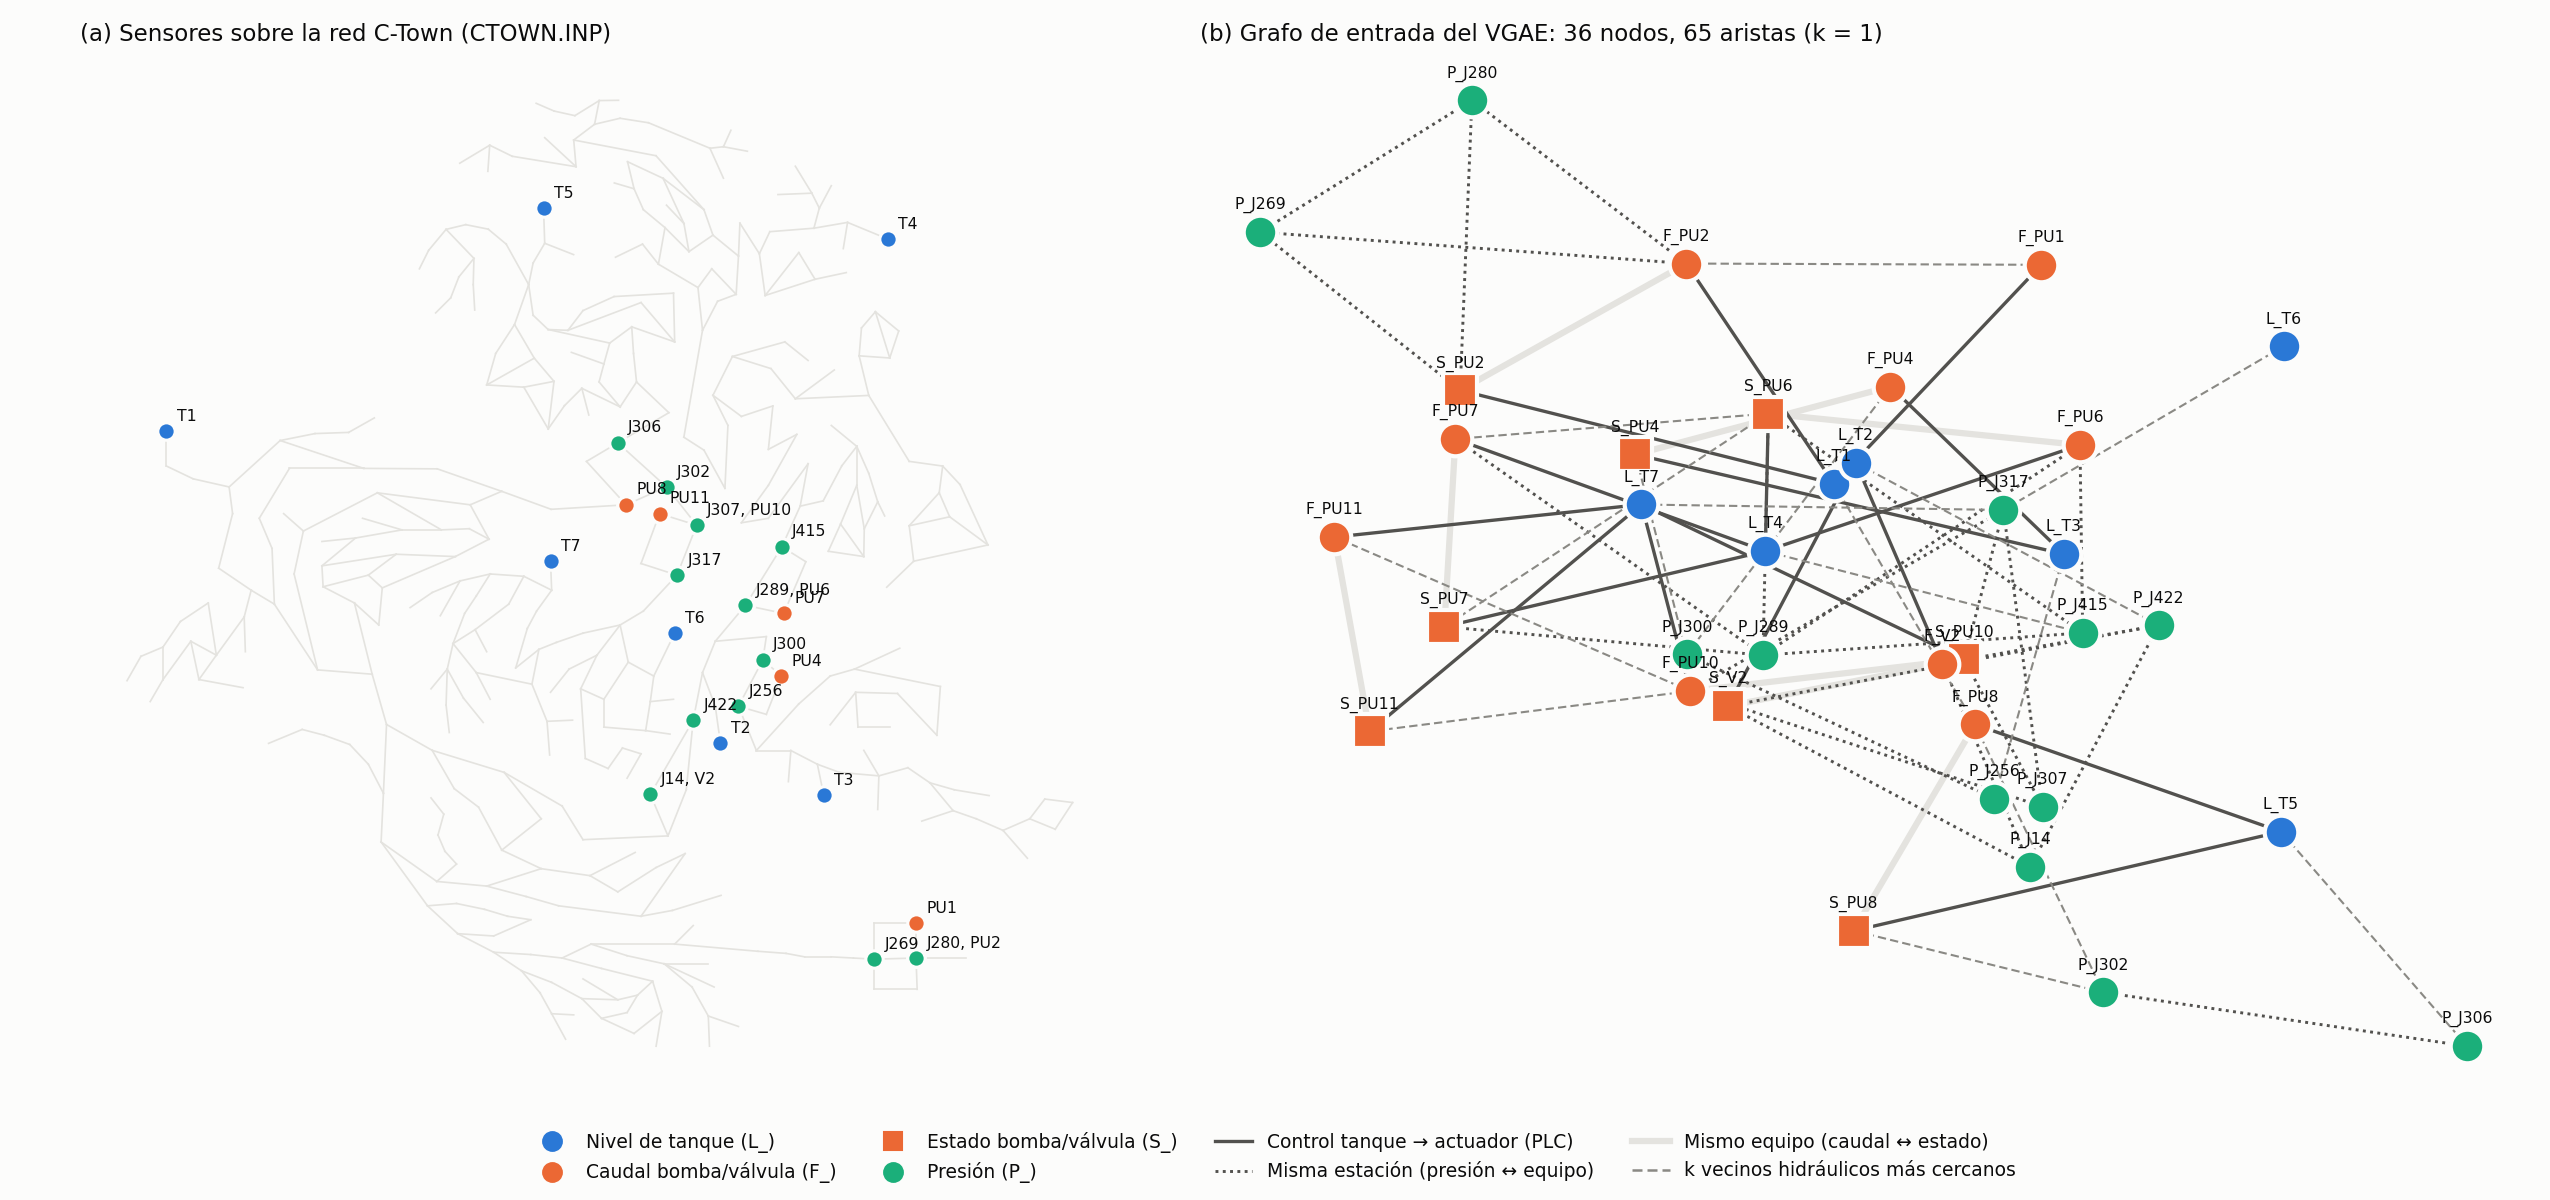
\includegraphics[width=\textwidth]{grafo_sensores.png}
\caption{(a) Ubicación de los sensores en la red C-Town. (b) Grafo de entrada del
VGAE con los cuatro tipos de arista.}
\label{fig:grafo}
\end{figure}

\subsection{Variational Graph Autoencoder para atributos de nodo}

Usamos la convolución de grafos de Kipf y Welling~\cite{kipf2017},
$\mathbf{H}^{(l+1)}=\sigma(\Ahat\mathbf{H}^{(l)}\mathbf{W}^{(l)})$ con
$\Ahat=\tilde{\mathbf{D}}^{-1/2}(\A+\mathbf{I})\tilde{\mathbf{D}}^{-1/2}$. El VGAE
original~\cite{kipf2016}, extensión a grafos del autoencoder
variacional~\cite{kingma2014}, codifica cada nodo en una gaussiana latente y
reconstruye solo la estructura. Como aquí el grafo es fijo y lo que cambia en el tiempo
son los atributos, introducimos tres modificaciones: (a) un decoder de atributos,
también GCN, que reconstruye la ventana de cada sensor; (b) \emph{embeddings}
aprendidos por nodo $\mathbf{e}_i\in\R^{d_e}$, que rompen la invariancia a
permutaciones de la GCN y permiten distinguir, por ejemplo, una presión de un nivel de
tanque; y (c) el decoder de producto interno original se conserva con peso pequeño
como regularizador topológico. La arquitectura (Figura~\ref{fig:arq}) es:
\begin{align}
\mathbf{H} &= \mathrm{ReLU}\big(\Ahat\,[\X\,\|\,\mathbf{E}]\,\mathbf{W}_1\big), \\
\bm\mu &= \Ahat\,\mathbf{H}\mathbf{W}_\mu,\qquad
\log\bm\sigma^2 = \Ahat\,\mathbf{H}\mathbf{W}_\sigma, \\
\Z &= \bm\mu+\bm\sigma\odot\bm\varepsilon,\quad \bm\varepsilon\sim\mathcal N(\mathbf 0,\mathbf I)
\quad(\Z=\bm\mu\ \text{en inferencia}), \\
\hat{\X} &= \mathrm{ReLU}\big(\Ahat\,[\Z\,\|\,\mathbf{E}]\,\mathbf{W}_d\big)\mathbf{W}_o,
\qquad \hat A_{ij}=\sigma(\mathbf z_i^\top\mathbf z_j).
\end{align}
Con la configuración seleccionada el modelo tiene 20\,364 parámetros. La pérdida es el
negativo de una ELBO ponderada:
\begin{equation}
\mathcal{L} = \frac{1}{NW}\big\|\X-\hat{\X}\big\|_F^2
+\alpha\,\mathrm{BCE}_{w}\big(\A,\sigma(\Z\Z^\top)\big)
+\frac{\beta}{N}\sum_{i=1}^{N}\KL\big(q(\mathbf{z}_i)\,\|\,\mathcal{N}(\mathbf{0},\mathbf{I})\big),
\label{eq:loss}
\end{equation}
donde la entropía cruzada se pondera para compensar la dispersión del grafo. Como el
decoder es una GCN, la reconstrucción de un sensor depende del estado latente de sus
vecinos: una lectura falsificada que no concuerda con su entorno produce un error
localizado en ese nodo, y una lectura reproducida (\emph{replay}) que sí parece normal
deja huella en los nodos vecinos cuyo comportamiento real sí cambió.

\begin{figure}[t]
\centering
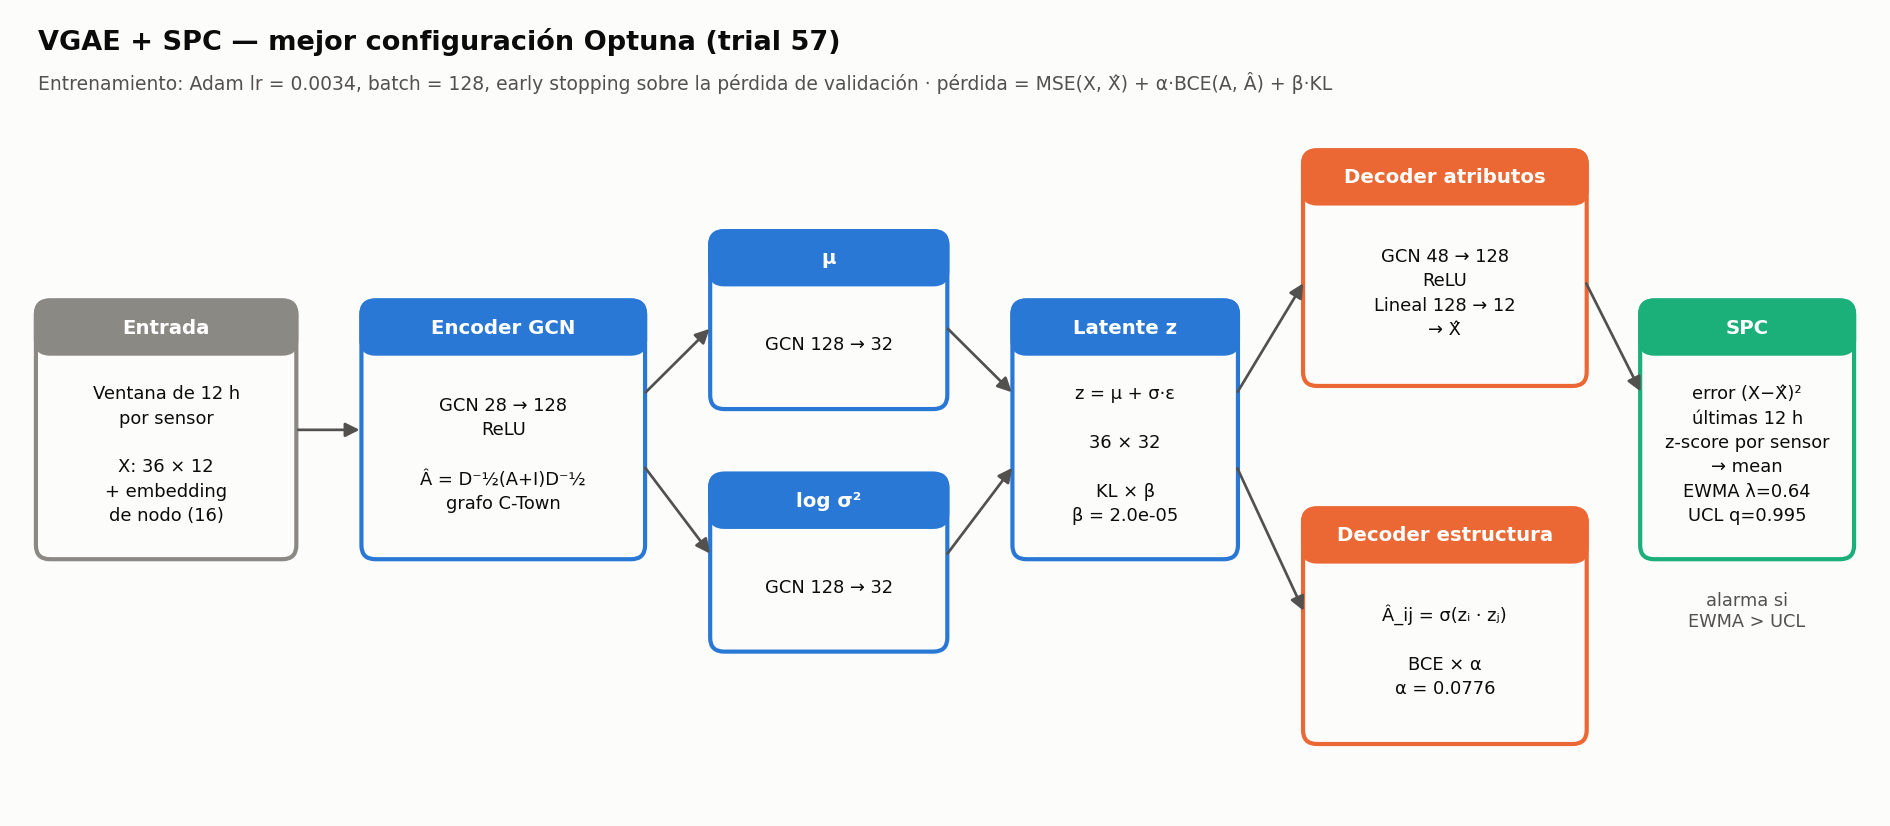
\includegraphics[width=\textwidth]{arquitectura_vgae.png}
\caption{Arquitectura VGAE + SPC con la configuración seleccionada por Optuna. El
bloque SPC muestra la carta EWMA de la búsqueda ($L=12$, $\lambda=0.64$,
$q=0.995$); en la comparación de cartas sus parámetros se reajustan
(Sección~\ref{sec:diseno}).}
\label{fig:arq}
\end{figure}

\subsection{Monitoreo con control estadístico de procesos}

Las cartas se calibran en \emph{Fase~I} (20\,\% final de \texttt{dataset03}, operación
normal no usada para ajustar pesos) y se aplican en \emph{Fase~II}. Siguiendo el MSPC
basado en PCA, se vigilan dos aspectos complementarios del VGAE: el residuo, que
detecta la pérdida de coherencia física entre sensores (p.\,ej.\ un nivel de tanque
falsificado que no concuerda con los caudales de sus bombas), y el espacio latente,
que detecta una operación físicamente coherente pero en un régimen inusual, caso
típico de la manipulación de actuadores o consignas.

\paragraph{Estadístico de residuo por sensor.} Sea
$\mathbf R_t=(\X_t-\hat\X_t)^{\odot2}$. Para cada sensor se promedia el error de las
últimas $L$ horas, se toma logaritmo y se estandariza con media $m_i$ y desviación
$s_i$ de Fase~I:
\begin{equation}
z_{t,i}=\frac{\log\!\big(\tfrac1L\textstyle\sum_{\ell=W-L+1}^{W}R_{t,i\ell}+10^{-6}\big)-m_i}{s_i}.
\label{eq:z}
\end{equation}
El logaritmo reduce la asimetría del error cuadrático y la estandarización hace
comparables sensores con niveles de error muy distintos, de modo que un ataque
localizado no se diluye entre los 36 nodos. Los $z_{t,i}$ se agregan en un escalar
$s_t$ mediante la media, el máximo o la media de los tres mayores.

\paragraph{Carta EWMA sobre el residuo.} $C_t=\lambda s_t+(1-\lambda)C_{t-1}$, con
$C_0=\bar s_{\text{F.I}}$ y $\lambda\in(0,1]$. Los ataques de BATADAL, en particular
los que ocultan la manipulación, producen desviaciones moderadas que se sostienen
durante horas o días, para las que las cartas con memoria son más
sensibles~\cite{montgomery2019}. La carta de Shewhart es el caso particular
$\lambda=1$; como ese valor se incluye en la búsqueda de $\lambda$, no se trata como
una carta aparte, pero se reporta como referencia sin memoria. No se incluye la CUSUM,
cuyo desempeño ante desplazamientos pequeños y sostenidos es prácticamente equivalente
al de la EWMA~\cite{lucas1990} y que añadiría otro parámetro que ajustar con los mismos
siete ataques.

\paragraph{Carta $T^2$ sobre el espacio latente.} Con el \emph{embedding} del grafo
$\bar{\bm\mu}_t=\frac1N\sum_i\bm\mu_{t,i}$ se calcula
$T^2_t=(\bar{\bm\mu}_t-\mathbf m)^\top\mathbf S^{+}(\bar{\bm\mu}_t-\mathbf m)$ con media
y covarianza de Fase~I.

\paragraph{Carta SPE.} Como referencia clásica del MSPC se incluye el estadístico $Q$
sin estandarizar, $Q_t=\sum_i \frac1L\sum_\ell R_{t,i\ell}$, con el límite de
Box~\cite{box1954,nomikos1995} $\UCL=g\,\chi^2_h(q)$, $g=v/2m$, $h=2m^2/v$, donde $m$ y
$v$ son la media y la varianza de $Q$ en Fase~I.

\paragraph{Límites y regla combinada.} Las ventanas consecutivas comparten $W-1$
horas, por lo que las series monitoreadas están fuertemente autocorrelacionadas y los
límites teóricos para observaciones independientes producirían un exceso de falsas
alarmas. Para la EWMA y el $T^2$ el límite es el cuantil empírico $q$ de la carta en
Fase~I, $\UCL=Q_q(\{C_t\}_{\text{F.I}})$, lo que fija una tasa nominal de falsas
alarmas $1-q$. Siguiendo la práctica del MSPC de vigilar residuo y subespacio a la vez,
el detector propuesto es la regla EWMA~$\vee$~$T^2$, que alarma si cualquiera de las
dos cartas supera su límite.

%=====================================================================
\section{Diseño experimental}
\label{sec:diseno}
%=====================================================================

\paragraph{Métrica.} Se usa la métrica oficial de BATADAL~\cite{taormina2018},
$S=\gamma\,S_{\mathrm{TTD}}+(1-\gamma)\,S_{\mathrm{CM}}$ con $\gamma=0.5$, donde
$S_{\mathrm{TTD}}=1-\frac1{n_A}\sum_a \mathrm{TTD}_a/\Delta t_a$ (TTD: horas desde el
inicio del ataque hasta la primera alarma dentro de su ventana; $\Delta t_a$ si no se
detecta) y $S_{\mathrm{CM}}=(\mathrm{TPR}+\mathrm{TNR})/2$ a nivel horario. Se reportan
además precisión, $F_1$ y número de ataques detectados.

\paragraph{Entrenamiento.} Adam sobre las ventanas del 80\,\% inicial de
\texttt{dataset03}, hasta 300 épocas con \emph{early stopping} (paciencia 25) sobre el
20\,\% final, restaurando los mejores pesos. En la práctica el criterio de parada casi
nunca se activó: la mediana de épocas en los ensayos de la búsqueda fue 300 y el
modelo final alcanzó su mejor pérdida de validación en la época 297.

\paragraph{Selección de hiperparámetros.} Los hiperparámetros del VGAE y de la carta
EWMA se seleccionan conjuntamente con Optuna~\cite{akiba2019} maximizando $S$ en
\texttt{dataset04} (Tabla~\ref{tab:espacio}). El estudio principal usa TPE
multivariante~\cite{bergstra2011} con 100 ensayos (10 aleatorios iniciales). Como
controles se ejecutan: (i) una búsqueda aleatoria de 50 ensayos con el mismo espacio,
comparada con TPE mediante la prueba U de Mann--Whitney unilateral; (ii) la importancia
de hiperparámetros por fANOVA~\cite{hutter2014}; y (iii) el reentrenamiento de la
mejor configuración TPE, la mejor aleatoria y la configuración por defecto con 10
semillas nuevas (100--109), contrastadas con la prueba de Wilcoxon pareada por semilla.
El conjunto de prueba se evalúa por primera vez en la etapa (iii).

\begin{table}[t]
\centering
\caption{Espacio de búsqueda, configuración por defecto y configuración seleccionada por TPE.}
\label{tab:espacio}
\small
\begin{tabular}{@{}lllll@{}}
\toprule
Grupo & Hiperparámetro & Espacio & Defecto & TPE \\
\midrule
Entrada y grafo & Ventana $W$ (h) & $\{12,24,48\}$ & 24 & 12 \\
 & Vecinos hidráulicos $k$ & $\{1,\dots,5\}$ & 3 & 1 \\
Arquitectura & Capa oculta $h$ & $\{32,64,128\}$ & 64 & 128 \\
 & Dimensión latente $d_z$ & $\{4,8,16,32\}$ & 16 & 32 \\
 & \emph{Embedding} de nodo $d_e$ & $\{4,8,16\}$ & 8 & 16 \\
Entrenamiento & Tasa de aprendizaje & $[10^{-4},5\cdot10^{-3}]$ (log) & $10^{-3}$ & $3.36\cdot10^{-3}$ \\
 & Tamaño de lote & $\{128,256,512\}$ & 64$^{\dagger}$ & 128 \\
 & Peso estructura $\alpha$ & $[10^{-3},1]$ (log) & 0.1 & 0.078 \\
 & Peso KL $\beta$ & $[10^{-5},10^{-1}]$ (log) & $10^{-3}$ & $2.0\cdot10^{-5}$ \\
Carta EWMA & Horizonte $L$ (h) & $\{1,3,6,12\}$ & 6 & 12 \\
 & Agregación & \{mean, max, top3\} & mean & mean \\
 & $\lambda$ & $[0.05,1]$ (log) & 0.2 & 0.645 \\
 & Cuantil $q$ & $\{0.99,0.995,0.999\}$ & 0.99 & 0.995 \\
\bottomrule
\multicolumn{5}{@{}p{0.95\textwidth}@{}}{\footnotesize $^{\dagger}$La configuración por
defecto se fijó antes de la búsqueda; el espacio de tamaños de lote se definió después
para aprovechar la GPU y no incluye el valor 64.}
\end{tabular}
\end{table}

\paragraph{Comparación de cartas.} Con el VGAE final, los parámetros de cada carta se
reajustan por búsqueda en rejilla sobre \texttt{dataset04}, pues los pesos finales del
modelo difieren de los del ensayo de Optuna: para la EWMA, $L\in\{1,3,6,12\}$,
agregación $\in\{$mean, max, top3$\}$, $\lambda\in\{0.05,0.1,0.2,0.5,1\}$ y
$q\in\{0.99,0.995,0.999\}$; para el $T^2$, $q$; y para SPE, $L\in\{1,3,6,12,24\}$ y $q$.
Se reportan además dos referencias: la mejor configuración de la rejilla con
$\lambda=1$ (carta de Shewhart) y la EWMA con los parámetros de Optuna. Cada
configuración se aplica sin cambios al conjunto de prueba.

\paragraph{Variante temporal.} Se evalúa una variante que sustituye la capa lineal de
entrada y salida por bloques convolucionales 1D dilatados ($d\in\{1,2,4\}$, campo
receptivo de 15~h) con codificación circular de la hora del día, en la línea de
STGCN~\cite{yu2018} y TCN~\cite{bai2018} (71\,185 parámetros). Se compara con el modelo
base en un diseño pareado: mismos hiperparámetros (los de Optuna), mismo grafo, mismo
presupuesto de entrenamiento (300 épocas, paciencia 25), mismas 10 semillas
(100--109) y la carta EWMA con los parámetros de Optuna; la única diferencia es el
bloque temporal. Como los hiperparámetros se eligieron para el modelo base, la
comparación es conservadora respecto de la variante.

%=====================================================================
\section{Resultados}
%=====================================================================

\subsection{Selección de hiperparámetros}

La búsqueda TPE alcanzó su mejor valor, $S=0.879$ en \texttt{dataset04}, en el ensayo
57, frente a $0.751$ de la mejor configuración aleatoria. La mediana de $S$ por ensayo
fue $0.802$ para TPE (ensayos guiados) y $0.586$ para la búsqueda aleatoria
(Mann--Whitney, $U=4294$, $p=3.1\cdot10^{-19}$). Según fANOVA, en el estudio TPE la
agregación del estadístico explica el 45.5\,\% de la varianza de $S$, seguida de la
ventana $W$ (17.4\,\%) y la dimensión latente (15.0\,\%); el resto de
hiperparámetros explica menos del 4\,\% cada uno. En la búsqueda aleatoria domina
$\lambda$ (56.7\,\%), lo que indica que, fuera de la región favorable, la memoria de
la carta es el factor que más condiciona el desempeño.

La Tabla~\ref{tab:semillas} muestra que la ventaja se mantiene al reentrenar con
semillas nuevas y se transfiere al conjunto de prueba. La configuración TPE supera a
la configuración por defecto y a la mejor aleatoria (Wilcoxon unilateral,
$p=0.00098$, el mínimo alcanzable con 10 pares), con una dispersión entre semillas
menor.

\begin{table}[t]
\centering
\caption{Robustez frente a la semilla: media $\pm$ desviación sobre 10 semillas (100--109), carta EWMA con los parámetros de cada configuración.}
\label{tab:semillas}
\small
\resizebox{\textwidth}{!}{%
\begin{tabular}{@{}lcccccc@{}}
\toprule
 & \multicolumn{2}{c}{\texttt{dataset04}} & \multicolumn{4}{c}{Prueba} \\
\cmidrule(lr){2-3}\cmidrule(l){4-7}
Configuración & $S$ & $F_1$ & $S$ & TPR & TNR & $F_1$ \\
\midrule
TPE (mejor)       & $\mathbf{0.852\pm0.014}$ & $\mathbf{0.676\pm0.006}$ & $\mathbf{0.750\pm0.017}$ & $\mathbf{0.426\pm0.026}$ & $\mathbf{0.976\pm0.005}$ & $\mathbf{0.557\pm0.020}$ \\
Aleatoria (mejor) & $0.704\pm0.034$ & $0.578\pm0.017$ & $0.496\pm0.062$ & $0.197\pm0.092$ & $0.972\pm0.004$ & $0.292\pm0.117$ \\
Por defecto       & $0.722\pm0.052$ & $0.592\pm0.014$ & $0.529\pm0.035$ & $0.185\pm0.022$ & $0.968\pm0.002$ & $0.281\pm0.028$ \\
\bottomrule
\end{tabular}}
\end{table}

\begin{figure}[t]
\centering
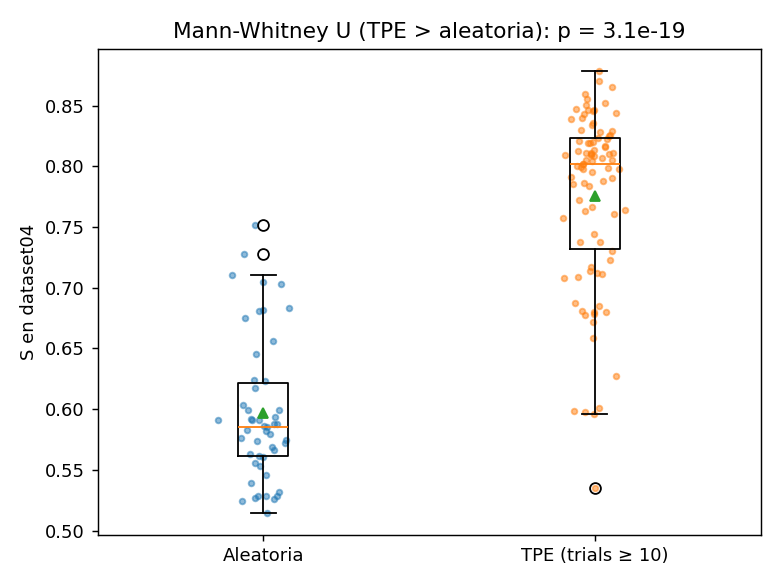
\includegraphics[width=0.49\textwidth]{tpe_vs_random.png}\hfill
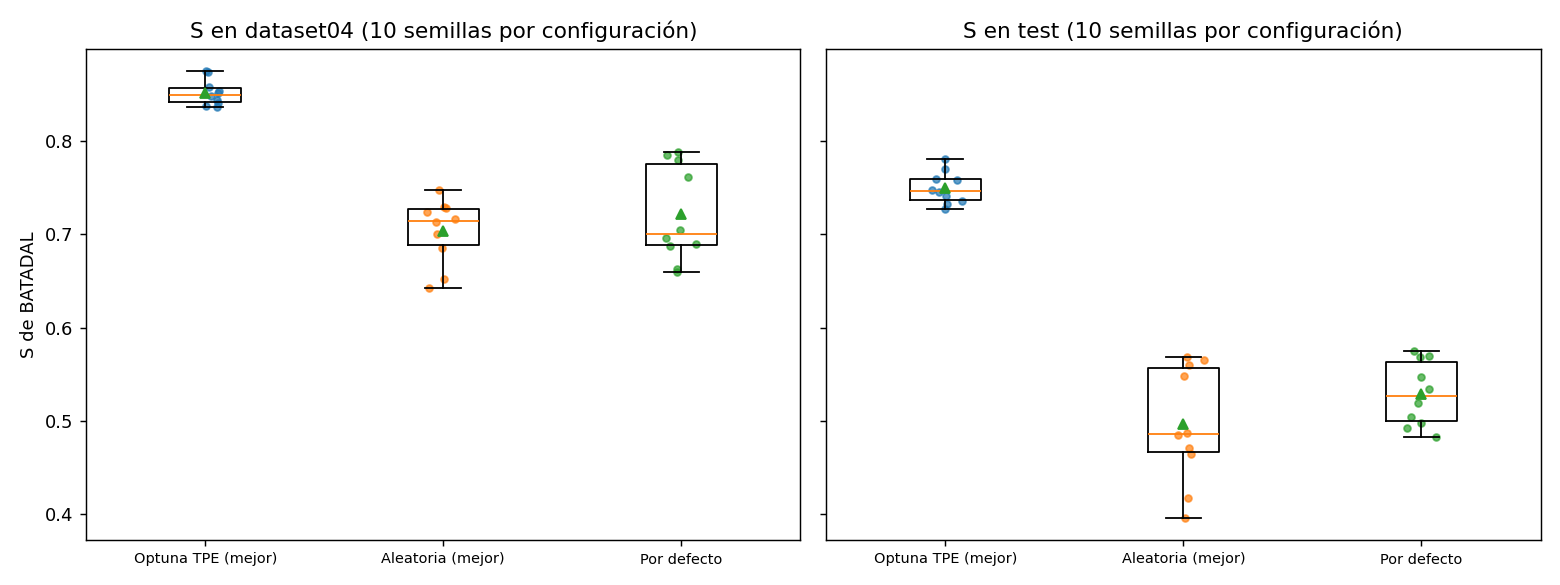
\includegraphics[width=0.49\textwidth]{seeds.png}
\caption{Izquierda: distribución de $S$ en \texttt{dataset04} por ensayo, TPE frente a
búsqueda aleatoria. Derecha: $S$ por semilla para las tres configuraciones.}
\label{fig:optuna}
\end{figure}

\subsection{Comparación de cartas de control}

El modelo final se entrenó con la configuración TPE y la semilla 0. Con la EWMA de
Optuna obtiene $S=0.722$ en prueba, ligeramente por debajo del rango observado con
las 10 semillas de la Tabla~\ref{tab:semillas} ($0.728$--$0.780$). La Tabla~\ref{tab:cartas} resume el
desempeño de cada carta y la Figura~\ref{fig:spc} muestra su evolución sobre el
conjunto de prueba.

\begin{table}[t]
\centering
\caption{Desempeño de las cartas con el VGAE final. Parámetros elegidos en \texttt{dataset04} y aplicados sin cambios a prueba. Det.: ataques detectados de 7. EWMA $\lambda{=}1$: mejor configuración de la rejilla sin memoria (carta de Shewhart).}
\label{tab:cartas}
\small
\setlength{\tabcolsep}{4pt}
\resizebox{\textwidth}{!}{%
\begin{tabular}{@{}llccccccccc@{}}
\toprule
Conjunto & Carta & Parámetros & $S$ & $S_{\mathrm{TTD}}$ & $S_{\mathrm{CM}}$ & TPR & TNR & Prec. & $F_1$ & Det. \\
\midrule
\multirow{6}{*}{\texttt{dataset04}}
 & EWMA & $L{=}3$, mean, $\lambda{=}0.1$ & 0.903 & 0.942 & 0.863 & 0.833 & 0.893 & 0.511 & 0.633 & 7 \\
 & EWMA $\lambda{=}1$ & $L{=}12$, max & 0.887 & \textbf{0.970} & 0.805 & \textbf{0.854} & 0.756 & 0.318 & 0.464 & 7 \\
 & EWMA (Optuna) & $L{=}12$, $\lambda{=}0.645$ & 0.837 & 0.886 & 0.788 & 0.604 & 0.973 & 0.748 & \textbf{0.668} & 7 \\
 & $T^2$ & --- & 0.729 & 0.705 & 0.754 & 0.533 & 0.976 & 0.744 & 0.621 & 7 \\
 & SPE & $L{=}6$ & 0.623 & 0.545 & 0.701 & 0.411 & \textbf{0.991} & \textbf{0.852} & 0.554 & 6 \\
 & EWMA $\vee$ $T^2$ & --- & \textbf{0.908} & 0.952 & \textbf{0.865} & 0.841 & 0.889 & 0.503 & 0.630 & 7 \\
\midrule
\multirow{6}{*}{Prueba}
 & EWMA & $L{=}3$, mean, $\lambda{=}0.1$ & 0.765 & 0.776 & 0.754 & 0.575 & 0.934 & 0.678 & 0.622 & 7 \\
 & EWMA $\lambda{=}1$ & $L{=}12$, max & \textbf{0.855} & \textbf{0.960} & 0.749 & \textbf{0.727} & 0.772 & 0.435 & 0.545 & 7 \\
 & EWMA (Optuna) & $L{=}12$, $\lambda{=}0.645$ & 0.722 & 0.765 & 0.679 & 0.378 & 0.979 & \textbf{0.815} & 0.517 & 7 \\
 & $T^2$ & --- & 0.678 & 0.744 & 0.613 & 0.243 & 0.983 & 0.773 & 0.370 & 7 \\
 & SPE & $L{=}6$ & 0.356 & 0.192 & 0.520 & 0.044 & \textbf{0.996} & 0.720 & 0.083 & 2 \\
 & EWMA $\vee$ $T^2$ & --- & 0.819 & 0.848 & \textbf{0.790} & 0.651 & 0.929 & 0.688 & \textbf{0.669} & 7 \\
\bottomrule
\multicolumn{11}{@{}l@{}}{\footnotesize Cuantil $q=0.99$ en todas las cartas salvo EWMA (Optuna), con $q=0.995$.}
\end{tabular}}
\end{table}

Cuatro resultados destacan:
\begin{enumerate}[leftmargin=*]
\item \textbf{El estadístico estandarizado por sensor es decisivo.} Las cartas
  construidas sobre $z_{t,i}$ detectan los 7 ataques en ambos conjuntos, mientras que
  la carta SPE, que suma el error crudo, detecta 6 de 7 en \texttt{dataset04} y solo 2
  de 7 en prueba ($S=0.356$): unos pocos sensores difíciles de reconstruir dominan
  $Q_t$ y enmascaran los ataques localizados.
\item \textbf{Residuo y latente son complementarios.} El $T^2$ es la carta más
  conservadora entre las que detectan los 7 ataques (TNR $0.983$), pero aporta
  detecciones tempranas donde el residuo tarda: en el ataque 12 la EWMA alarma a las
  48~h y el $T^2$ a las 7~h. La regla EWMA~$\vee$~$T^2$ mejora a la EWMA en prueba de
  $S=0.765$ a $0.819$ y obtiene el mejor $S_{\mathrm{CM}}$ y $F_1$ de todas las cartas.
\item \textbf{La memoria aporta en \texttt{dataset04}, pero la ventaja no se mantiene
  en $S$.} En \texttt{dataset04} la EWMA con $\lambda=0.1$ supera a la versión sin
  memoria ($0.903$ frente a $0.887$); en prueba el orden se invierte ($0.765$ frente a
  $0.855$).
\item \textbf{La carta sin memoria obtiene el mayor $S$ en prueba, pero con muchas
  falsas alarmas.} Su TNR es $0.772$: alarma en el 23\,\% de las horas normales,
  frente al 1\,\% nominal (Sección~\ref{sec:discusion}).
\end{enumerate}

\begin{figure}[p]
\centering
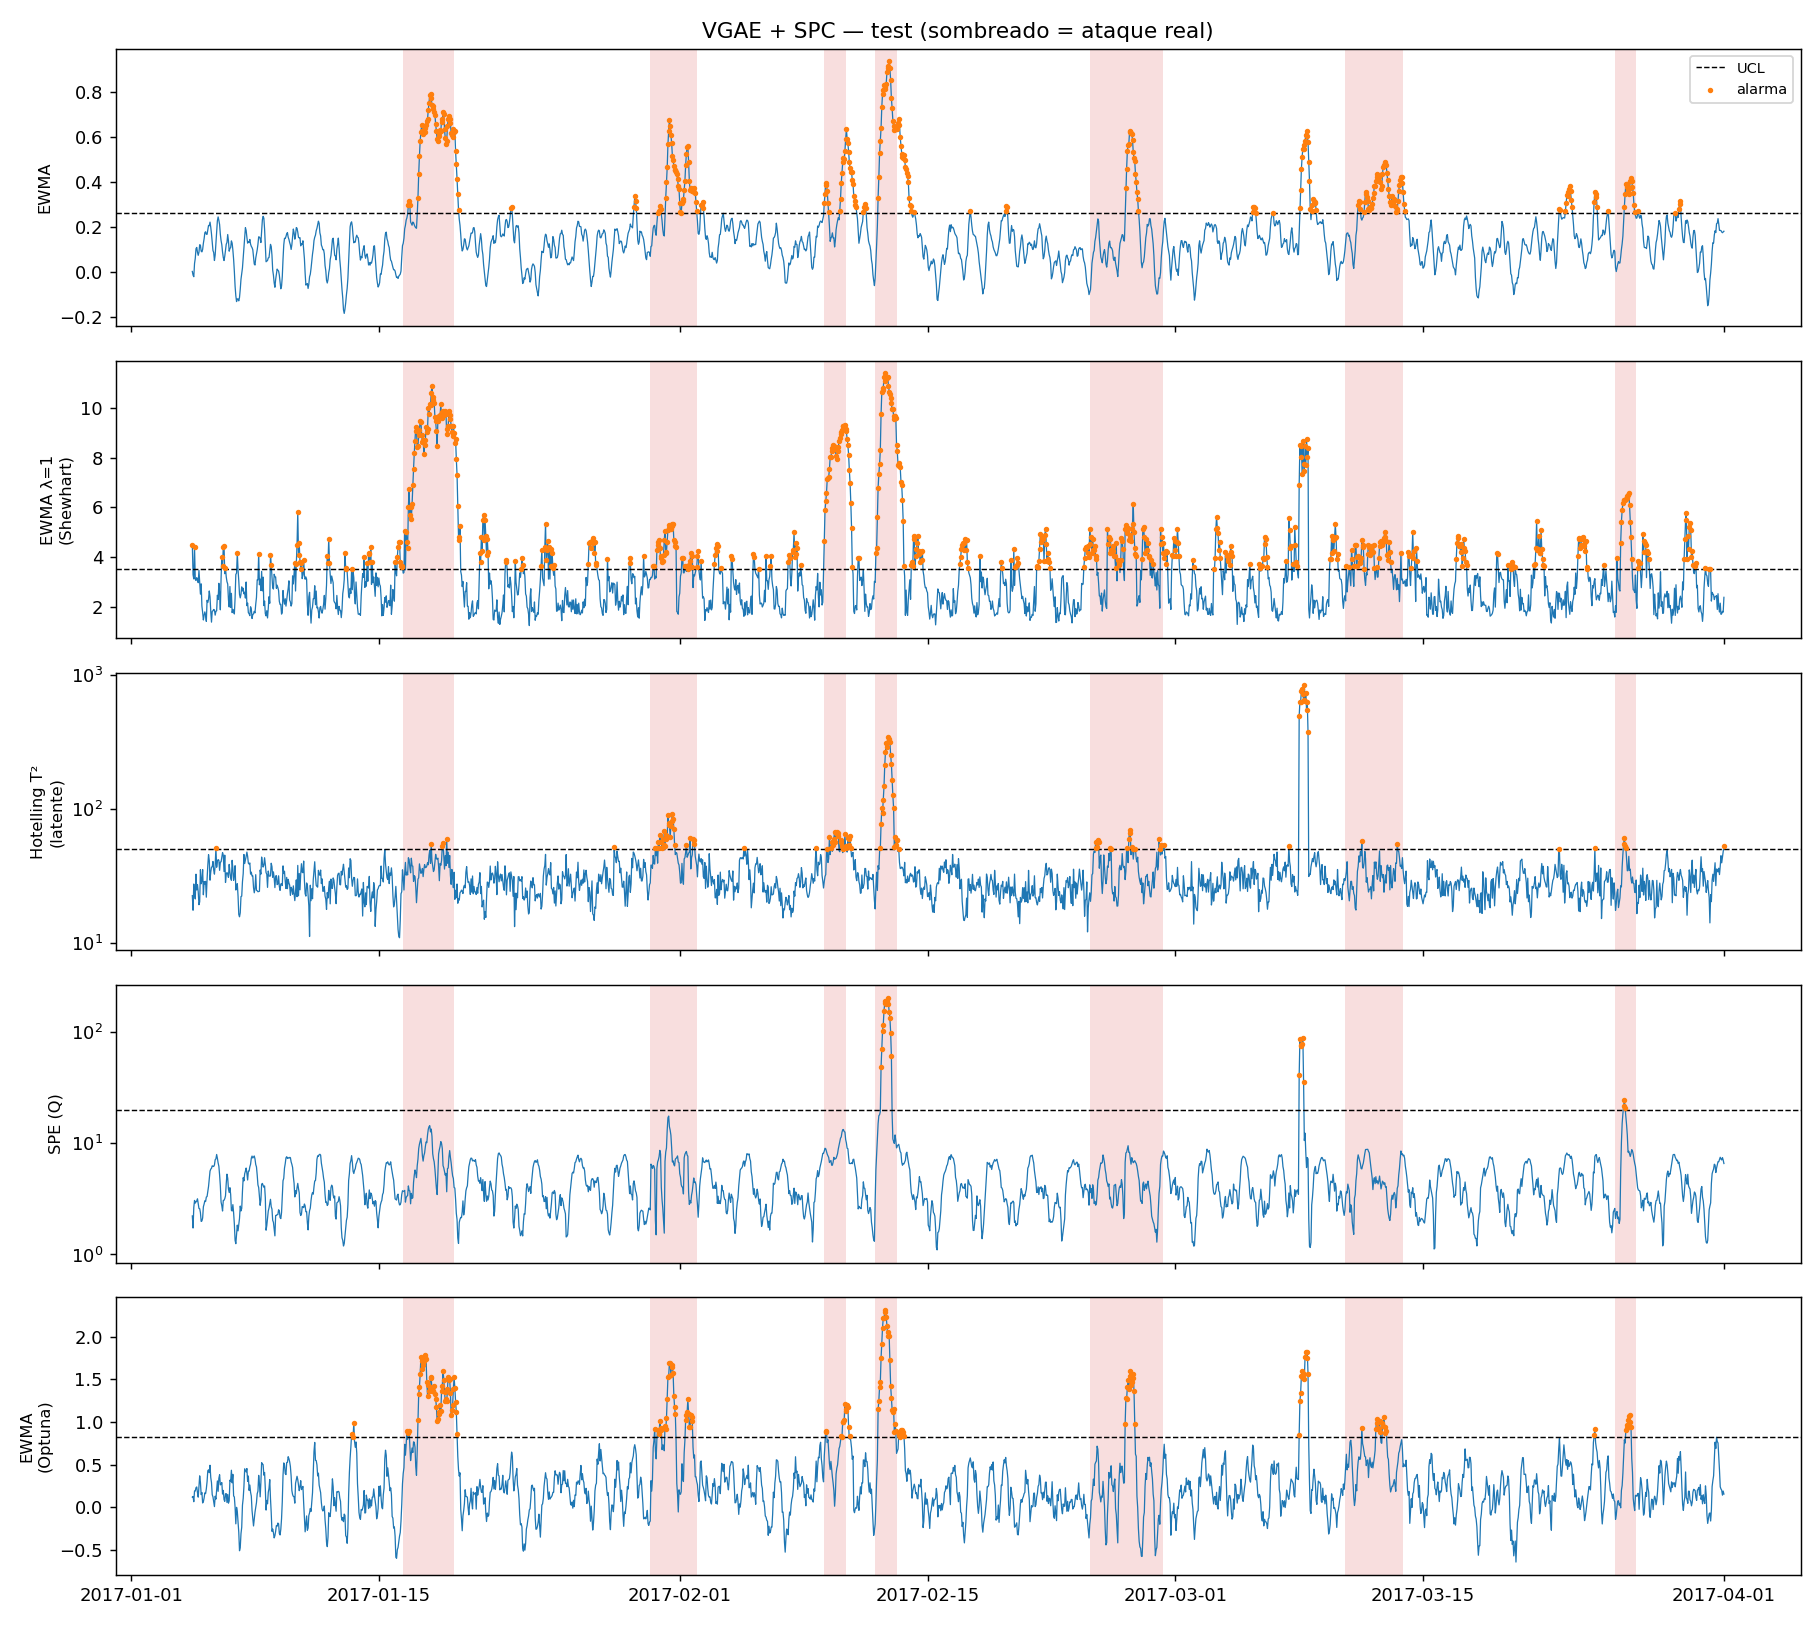
\includegraphics[width=\textwidth]{spc_test.png}
\caption{Cartas de control sobre el conjunto de prueba con el VGAE final. Sombreado:
ataques reales; línea discontinua: límite de control; puntos: alarmas. Escala
logarítmica simétrica en $T^2$ y SPE.}
\label{fig:spc}
\end{figure}

\subsection{Tiempo hasta la detección por ataque}

\begin{table}[t]
\centering
\caption{Tiempo hasta la detección (h) por ataque en el conjunto de prueba. ``---'': no detectado.}
\label{tab:ttd}
\small
\begin{tabular}{@{}crcccccc@{}}
\toprule
Ataque & Duración & EWMA & EWMA $\lambda{=}1$ & EWMA (Optuna) & $T^2$ & SPE & EWMA $\vee$ $T^2$ \\
\midrule
8  & 70  & 7  & 2 & 5  & 38 & --- & 7  \\
9  & 65  & 11 & 4 & 6  & 7  & --- & 7  \\
10 & 31  & 1  & 1 & 3  & 5  & --- & 1  \\
11 & 31  & 4  & 1 & 4  & 7  & 8   & 4  \\
12 & 100 & 48 & 0 & 47 & 7  & --- & 7  \\
13 & 80  & 18 & 2 & 23 & 23 & --- & 18 \\
14 & 30  & 13 & 3 & 15 & 12 & 12  & 12 \\
\bottomrule
\end{tabular}
\end{table}

La Tabla~\ref{tab:ttd} detalla los tiempos de detección. Los ataques 10 y 11
(activación de PU3, sin ocultamiento) se detectan en 1--4~h con todas las cartas
basadas en $z$. Los ataques con \emph{replay} (8, 12 y 13) son los más lentos para la
EWMA: en el 12 tarda casi la mitad del ataque. En ese caso el $T^2$ adelanta la
detección de la regla combinada de 48 a 7~h.

\subsection{Diagnóstico: qué sensores explican la alarma}

Como el estadístico~\eqref{eq:z} está definido por sensor, cada alarma puede
atribuirse a los nodos que más contribuyen a ella. La Figura~\ref{fig:nodos} muestra
el $z$ medio de cada sensor durante cada ataque de prueba. Para interpretarla hay que
tener en cuenta una línea base: en las horas normales de prueba, los sensores del
subsistema T1--PU1/PU2 ($S\_PU2$, $F\_PU2$, $F\_PU1$, $L\_T1$) tienen un $z$ medio de
1.4--1.9, frente a una mediana de 0.02 en el resto de sensores
(Sección~\ref{sec:discusion}). Por eso, valores de ese orden en esos sensores no
constituyen evidencia de ataque.

\begin{figure}[t]
\centering
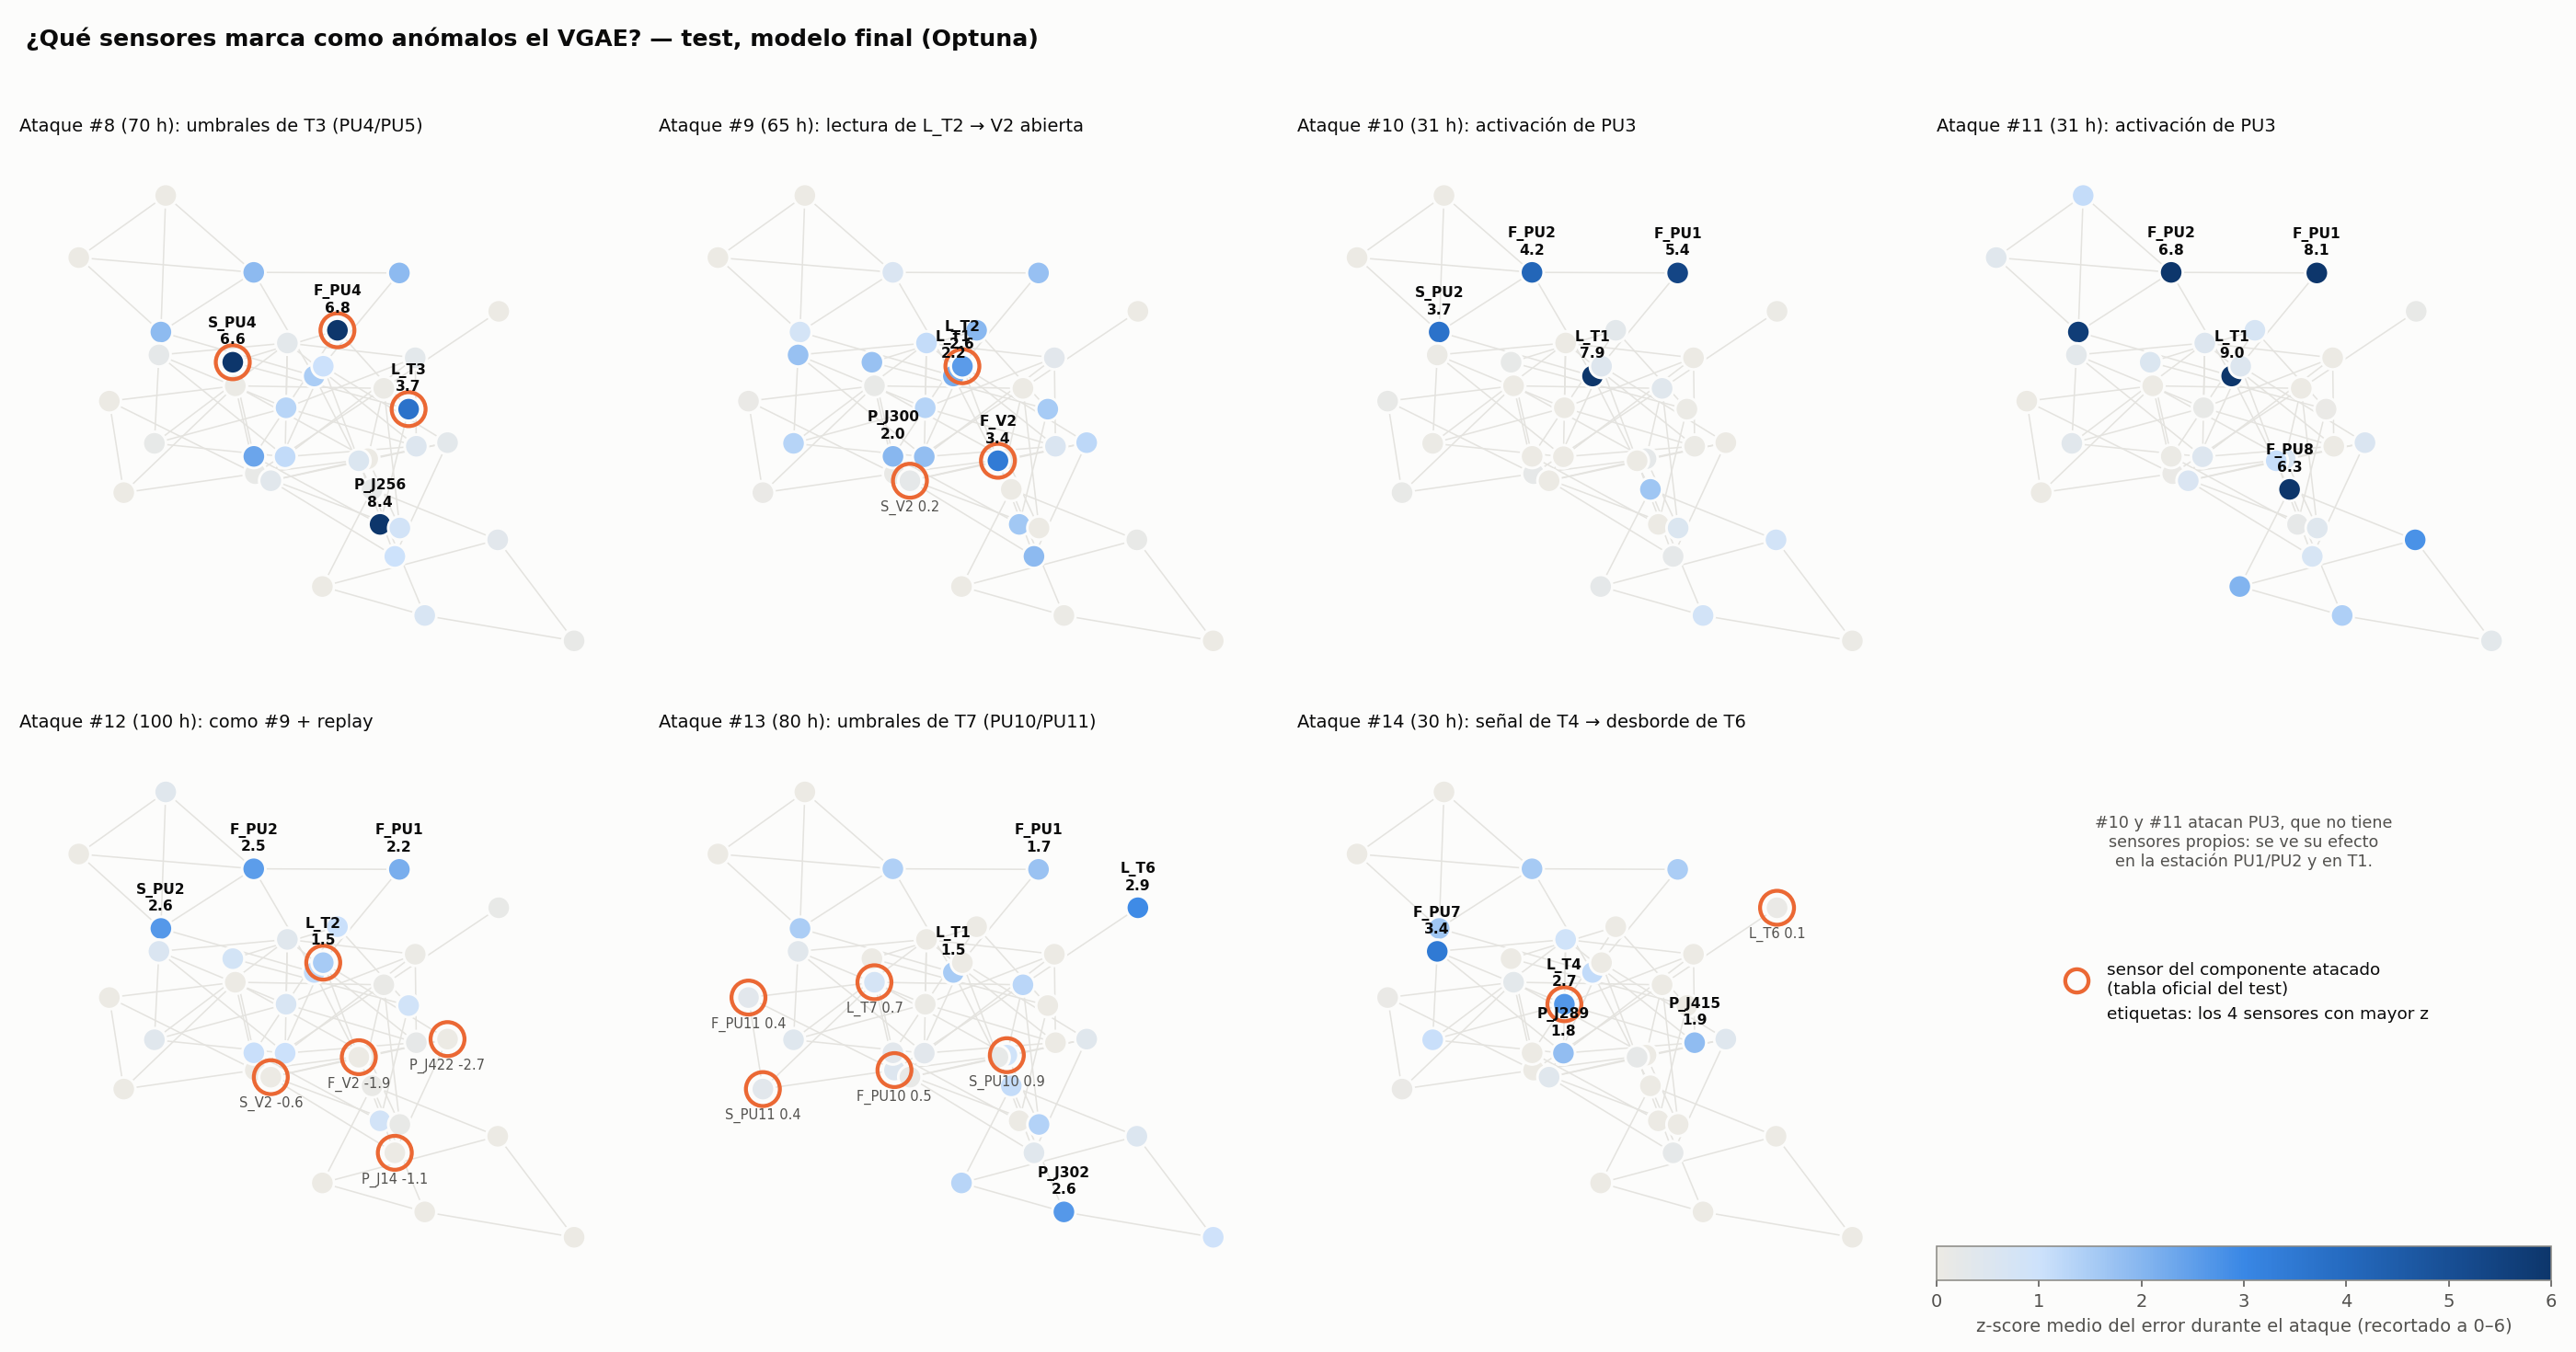
\includegraphics[width=\textwidth]{nodos_anomalos_test.png}
\caption{$z$ medio del error de reconstrucción por sensor durante cada ataque de
prueba, con el horizonte $L=12$~h de la configuración Optuna. Círculos: sensores del
componente atacado según la documentación oficial; etiquetas: los cuatro sensores
con mayor $z$.}
\label{fig:nodos}
\end{figure}

\begin{itemize}[leftmargin=*]
\item \textbf{Ataques sin ocultamiento o con ocultamiento parcial} (8, 9, 14): los
  sensores con mayor $z$ coinciden con el componente atacado o con su lazo de control
  ($P\_J256=8.4$, $F\_PU4=6.8$, $S\_PU4=6.6$ y $L\_T3=3.7$ en el ataque 8;
  $F\_V2=3.4$ y $L\_T2=2.6$ en el 9; $F\_PU7=3.4$ y $L\_T4=2.7$ en el 14).
\item \textbf{Componente sin sensores} (10, 11): PU3 no forma parte del modelo, pero
  su activación altera el tanque T1 y la estación PU1/PU2 ($L\_T1=7.9$ y $9.0$,
  $F\_PU1=5.4$ y $8.1$), muy por encima de la línea base de ese subsistema. La
  detección se apoya íntegramente en la propagación por el grafo.
\item \textbf{\emph{Replay}} (12, 13): los sensores reproducidos tienen $z$ bajo o
  negativo (p.\,ej.\ $F\_V2=-1.9$ y $P\_J422=-2.7$ en el ataque 12; 0.4--0.9 en los
  sensores de PU10/PU11 en el 13), porque muestran datos normales. En el ataque 13 la
  alarma proviene de efectos físicos que el atacante no ocultó ($L\_T6=2.9$,
  $P\_J302=2.6$). En el ataque 12 los $z$ más altos (2.2--2.6 en PU1/PU2) no superan
  la línea base; descontada esta, el sensor con mayor exceso es $L\_T2$ ($+1.6$), uno
  de los reproducidos, de modo que el diagnóstico de este ataque es débil.
\end{itemize}

El diagnóstico debe interpretarse, por tanto, como ``dónde se rompe la coherencia
física respecto a la operación normal reciente'' y no necesariamente como ``qué
sensor fue atacado'': en los ataques con \emph{replay}, los sensores del componente
atacado son precisamente los que parecen más normales.

\subsection{Variante con convolución temporal}

La Tabla~\ref{tab:temporal} y la Figura~\ref{fig:temporal} resumen la comparación
pareada con 10 semillas. La variante temporal obtiene una pérdida de validación menor
($0.149$ frente a $0.161$) y converge antes: el \emph{early stopping} la detiene en una
mediana de 170 épocas (rango 100--300), mientras que el modelo base agota las 300 en
todas las semillas. En detección, la variante mejora la $S$ media en prueba en
$+0.016$ y gana en 7 de 10 semillas, pero la diferencia no es significativa (Wilcoxon
bilateral, $p=0.13$); en \texttt{dataset04} la mejora es de $+0.011$ (6 de 10,
$p=0.19$). Gran parte de la diferencia media en prueba se debe a una sola semilla
(109, $+0.092$); la mediana de las diferencias es $+0.014$. La mejora proviene sobre
todo de la sensibilidad (TPR $0.465$ frente a $0.420$), con una TNR prácticamente igual.

\begin{table}[t]
\centering
\caption{Comparación pareada del VGAE base y la variante con convolución temporal:
media $\pm$ desviación sobre 10 semillas (100--109), 300 épocas con paciencia 25, carta
EWMA con los parámetros de Optuna.}
\label{tab:temporal}
\small
\resizebox{\textwidth}{!}{%
\begin{tabular}{@{}lcccccc@{}}
\toprule
 & & \texttt{dataset04} & \multicolumn{4}{c}{Prueba} \\
\cmidrule(lr){3-3}\cmidrule(l){4-7}
Modelo & Pérdida val. & $S$ & $S$ & TPR & TNR & $F_1$ \\
\midrule
VGAE base & $0.161\pm0.001$ & $0.855\pm0.018$ & $0.741\pm0.016$ & $0.420\pm0.026$ & $0.977\pm0.004$ & $0.553\pm0.022$ \\
+ conv.\ temporal & $0.149\pm0.005$ & $0.866\pm0.017$ & $0.758\pm0.025$ & $0.465\pm0.051$ & $0.973\pm0.006$ & $0.589\pm0.040$ \\
\midrule
Diferencia (gana) & --- & $+0.011$ (6/10) & $+0.016$ (7/10) & & & \\
Wilcoxon bilateral & --- & $p=0.19$ & $p=0.13$ & & & \\
\bottomrule
\end{tabular}}
\end{table}

\begin{figure}[t]
\centering
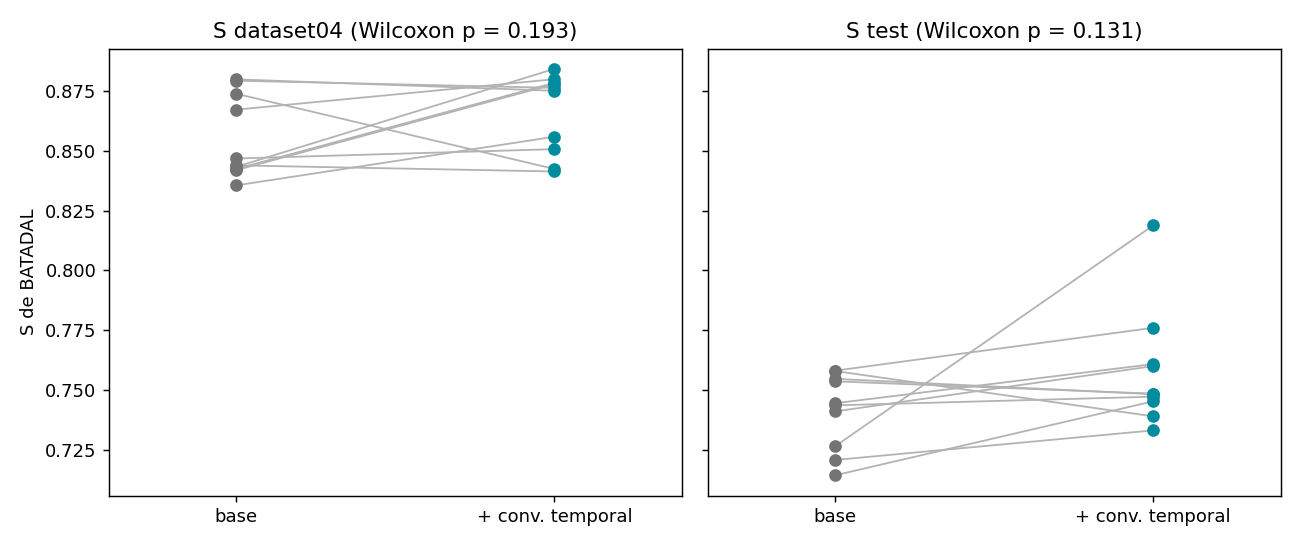
\includegraphics[width=0.8\textwidth]{seeds_temporal.png}
\caption{$S$ por semilla del VGAE base y de la variante con convolución temporal;
cada línea une los dos modelos entrenados con la misma semilla.}
\label{fig:temporal}
\end{figure}

Una comparación preliminar con solo 40 épocas había mostrado una ventaja mucho mayor
($+0.086$ en prueba con 2 semillas). Con el presupuesto completo la ventaja se reduce a
una quinta parte, lo que indica que procedía sobre todo de la convergencia más rápida
de la variante y no de una mejor capacidad de detección. El modelo base de esta
comparación coincide en configuración con la etapa de semillas de la
Tabla~\ref{tab:semillas} ($0.741\pm0.016$ frente a $0.750\pm0.017$ en prueba); la
pequeña diferencia es compatible con la variabilidad entre semillas y con haber
entrenado en CPU en lugar de GPU.

%=====================================================================
\section{Discusión}
\label{sec:discusion}
%=====================================================================

\paragraph{La métrica $S$ premia la densidad de alarmas.} El término
$S_{\mathrm{TTD}}$ solo mide la primera alarma dentro de cada ataque y no penaliza las
alarmas previas. Taormina et al.~\cite{taormina2018} ya señalan que $S$ está sesgada
hacia la detección: un detector que siempre alarma obtiene $S=0.75$. En nuestro caso,
con la tasa de falsas alarmas de la carta sin memoria en prueba
($1-\mathrm{TNR}=0.228$), una alarma cae en promedio cada $\approx4.4$~h aun sin
información sobre el ataque, lo que es del orden de sus TTD (0--4~h). Por ello su
$S_{\mathrm{TTD}}=0.960$ no debe leerse como evidencia de mayor sensibilidad. La regla
EWMA~$\vee$~$T^2$ ofrece un compromiso más útil para la operación: TNR de $0.929$,
precisión de $0.688$ y el mejor $F_1$. Recomendamos reportar siempre TNR, precisión y
$F_1$ junto a $S$.

\paragraph{La tasa nominal de falsas alarmas no se conserva.} Los límites se fijan en
el cuantil $q=0.99$ de Fase~I, pero las tasas observadas son del 10.7\,\%
(\texttt{dataset04}) y 6.6\,\% (prueba) para la EWMA, del 7.1\,\% para la regla
combinada en prueba y del 22.8\,\% para la carta sin memoria. Identificamos cuatro
causas:
\begin{enumerate}[leftmargin=*]
\item \textbf{Recuperación tras los ataques.} Las horas posteriores a un ataque
  cuentan como normales aunque el sistema aún se esté recuperando. En prueba, el
  43\,\% de las falsas alarmas de la EWMA cae en las 24~h siguientes al final de un
  ataque, un intervalo que contiene solo el 10\,\% de las horas normales.
\item \textbf{Deriva localizada en T1--PU1/PU2.} Los sensores de este subsistema
  tienen un $z$ medio de 1.1--1.6 ($L=3$) en las horas normales de \texttt{dataset04}
  y de prueba, mientras que la mediana del resto es $\approx0$. No se trata de un
  cambio general de régimen: Taormina et al.~\cite{taormina2018} indican que los
  patrones de demanda son regulares y consistentes entre los tres conjuntos, y el
  resto de sensores se mantiene en su nivel de Fase~I.
\item \textbf{Doble uso de la Fase~I.} El mismo tramo sirve para el \emph{early
  stopping} y para calibrar los límites. El modelo se elige para reconstruir bien esos
  datos, lo que estrecha los límites respecto de datos normales nuevos.
\item \textbf{Regla combinada sin recalibrar.} Cada carta usa su propio $q=0.99$, por
  lo que la tasa nominal de la unión es mayor que la de cada carta.
\end{enumerate}
Además, la Figura~\ref{fig:spc} muestra un evento sin ataque etiquetado (7--8 de marzo
de 2017) que $T^2$, SPE y EWMA señalan con fuerza: la bomba PU6 se activa durante 2~h,
un régimen que ocupa solo 16 de las 8\,761 horas de \texttt{dataset03}. Es una
operación legítima pero poco frecuente, que el detector, entrenado con datos normales,
no puede distinguir de un ataque.

\paragraph{La selección en \texttt{dataset04} y su transferencia.} \texttt{dataset04}
contiene solo 7 ataques, y el orden entre la EWMA y la carta sin memoria se invierte
entre \texttt{dataset04} y prueba. Parte de la diferencia se explica por las tasas de
falsas alarmas y el sesgo de $S$ descrito arriba. Por ello fijamos el detector
propuesto (EWMA~$\vee$~$T^2$) por argumentos de diseño ---la lógica residuo/latente del
MSPC--- y no por su $S$ en prueba; los datos de validación se usan solo para ajustar
sus parámetros.

\paragraph{Comparación con BATADAL.} La Tabla~\ref{tab:batadal} sitúa el detector
propuesto frente a los participantes de la competición, evaluados sobre el mismo
conjunto de prueba. Con $S=0.819$ quedaría en la quinta posición, por debajo de los
enfoques que combinan detección estadística con conocimiento del sistema. La
comparación debe tomarse con cautela por dos diferencias de protocolo que favorecen a
nuestro método: los participantes disponían de etiquetas parciales de
\texttt{dataset04}, mientras que nosotros seleccionamos hiperparámetros con las
ventanas completas reconstruidas tras la competición, y diseñamos el método conociendo
ya los resultados de la competición. En sentido contrario, nuestro detector no usa el
modelo hidráulico en línea ni datos de prueba sin etiquetar.

\begin{table}[t]
\centering
\caption{Comparación con los participantes de BATADAL en el conjunto de prueba (Tabla~4 de Taormina et al.~\cite{taormina2018}). $S_{\mathrm{CM}}$ corresponde a $S_{\mathrm{CLF}}$ en la notación original.}
\label{tab:batadal}
\small
\begin{tabular}{@{}lcccccc@{}}
\toprule
Método & Det. & $S$ & $S_{\mathrm{TTD}}$ & $S_{\mathrm{CM}}$ & TPR & TNR \\
\midrule
Housh y Ohar & 7 & 0.970 & 0.965 & 0.975 & 0.953 & 0.997 \\
Abokifa et al. & 7 & 0.949 & 0.958 & 0.940 & 0.921 & 0.959 \\
Giacomoni et al. & 7 & 0.927 & 0.936 & 0.917 & 0.838 & 0.997 \\
Brentan et al. & 6 & 0.894 & 0.857 & 0.931 & 0.889 & 0.973 \\
\textbf{VGAE + SPC (EWMA $\vee$ $T^2$)} & 7 & \textbf{0.819} & 0.848 & 0.790 & 0.651 & 0.929 \\
Chandy et al. & 7 & 0.802 & 0.835 & 0.768 & 0.857 & 0.678 \\
Pasha et al. & 7 & 0.773 & 0.885 & 0.660 & 0.329 & 0.992 \\
Aghashahi et al. & 3 & 0.534 & 0.429 & 0.640 & 0.396 & 0.884 \\
\bottomrule
\end{tabular}
\end{table}

\paragraph{Limitaciones.} (i) Los datos son simulados. (ii) La comparación de cartas
se hizo sobre un único modelo final; la variabilidad entre semillas de la EWMA de
Optuna es del orden de $\pm0.02$ en $S$ (Tabla~\ref{tab:semillas}), y diferencias entre
cartas de ese orden no deben interpretarse. (iii) Las ventanas consecutivas se solapan,
por lo que los límites empíricos se basan en una muestra efectiva mucho menor que las
1\,753 horas de Fase~I. (iv) El entrenamiento no llegó a converger dentro del
presupuesto de 300 épocas (mejor época 297), de modo que el modelo probablemente
mejoraría con más épocas.

%=====================================================================
\section{Conclusiones}
%=====================================================================

Hemos presentado un detector de ciberataques para redes de distribución de agua que
combina un VGAE sobre un grafo de sensores derivado de la física y del control de la
red con cartas de control estadístico de procesos. El modelo se entrena solo con
operación normal y produce alarmas interpretables a nivel de sensor. Con
hiperparámetros seleccionados por TPE, cuya ventaja sobre la búsqueda aleatoria y la
configuración por defecto es estadísticamente significativa y estable frente a la
semilla, la regla EWMA~$\vee$~$T^2$ detecta los 7 ataques de prueba de BATADAL con
$S=0.819$ y $F_1=0.669$. Tres hallazgos tienen alcance general: la estandarización del
residuo por sensor es imprescindible para detectar ataques localizados; vigilar a la
vez el residuo y el espacio latente aporta detecciones que ninguna carta logra por
separado; y la métrica de BATADAL puede favorecer detectores con alta densidad de
alarmas, por lo que debe acompañarse de TNR y precisión. Modelar explícitamente el
orden temporal con convoluciones dilatadas acelera la convergencia, pero con el
presupuesto completo no aporta una mejora significativa en la detección. Como trabajo
futuro se plantea separar la validación del \emph{early stopping} de la Fase~I, recalibrar los
límites de la regla combinada, estudiar la deriva del subsistema T1--PU1/PU2 y evaluar
el método en datos reales o en otros bancos de prueba como SWaT.

%=====================================================================
\begin{thebibliography}{99}
%=====================================================================
\bibitem{abokifa2019} Abokifa, A.\,A., Haddad, K., Lo, C. y Biswas, P. (2019).
  Real-time identification of cyber-physical attacks on water distribution systems via
  machine learning--based anomaly detection techniques. \emph{Journal of Water Resources
  Planning and Management}, 145(1).
\bibitem{akiba2019} Akiba, T., Sano, S., Yanase, T., Ohta, T. y Koyama, M. (2019).
  Optuna: A next-generation hyperparameter optimization framework. \emph{KDD}.
\bibitem{bai2018} Bai, S., Kolter, J.\,Z. y Koltun, V. (2018). An empirical evaluation
  of generic convolutional and recurrent networks for sequence modeling.
  \emph{arXiv:1803.01271}.
\bibitem{bergstra2011} Bergstra, J., Bardenet, R., Bengio, Y. y Kégl, B. (2011).
  Algorithms for hyper-parameter optimization. \emph{NeurIPS}.
\bibitem{box1954} Box, G.\,E.\,P. (1954). Some theorems on quadratic forms applied in
  the study of analysis of variance problems. \emph{Annals of Mathematical Statistics},
  25(2).
\bibitem{deng2021} Deng, A. y Hooi, B. (2021). Graph neural network-based anomaly
  detection in multivariate time series. \emph{AAAI}.
\bibitem{goh2016} Goh, J., Adepu, S., Junejo, K.\,N. y Mathur, A. (2016). A dataset to
  support research in the design of secure water treatment systems. \emph{CRITIS}.
\bibitem{housh2018} Housh, M. y Ohar, Z. (2018). Model-based approach for
  cyber-physical attack detection in water distribution systems. \emph{Water Research},
  139.
\bibitem{hundman2018} Hundman, K., Constantinou, V., Laporte, C., Colwell, I. y
  Soderstrom, T. (2018). Detecting spacecraft anomalies using LSTMs and nonparametric
  dynamic thresholding. \emph{KDD}.
\bibitem{hutter2014} Hutter, F., Hoos, H. y Leyton-Brown, K. (2014). An efficient
  approach for assessing hyperparameter importance. \emph{ICML}.
\bibitem{jackson1979} Jackson, J.\,E. y Mudholkar, G.\,S. (1979). Control procedures
  for residuals associated with principal component analysis. \emph{Technometrics},
  21(3).
\bibitem{kingma2014} Kingma, D.\,P. y Welling, M. (2014). Auto-encoding variational
  Bayes. \emph{ICLR}.
\bibitem{kipf2016} Kipf, T.\,N. y Welling, M. (2016). Variational graph auto-encoders.
  \emph{NeurIPS Workshop on Bayesian Deep Learning}.
\bibitem{kipf2017} Kipf, T.\,N. y Welling, M. (2017). Semi-supervised classification
  with graph convolutional networks. \emph{ICLR}.
\bibitem{kourti1995} Kourti, T. y MacGregor, J.\,F. (1995). Process analysis,
  monitoring and diagnosis, using multivariate projection methods.
  \emph{Chemometrics and Intelligent Laboratory Systems}, 28(1).
\bibitem{kravchik2018} Kravchik, M. y Shabtai, A. (2018). Detecting cyber attacks in
  industrial control systems using convolutional neural networks. \emph{CPS-SPC
  Workshop}.
\bibitem{lucas1990} Lucas, J.\,M. y Saccucci, M.\,S. (1990). Exponentially weighted
  moving average control schemes: properties and enhancements. \emph{Technometrics},
  32(1).
\bibitem{montgomery2019} Montgomery, D.\,C. (2019). \emph{Introduction to Statistical
  Quality Control} (8.\textsuperscript{a} ed.). Wiley.
\bibitem{nomikos1995} Nomikos, P. y MacGregor, J.\,F. (1995). Multivariate SPC charts
  for monitoring batch processes. \emph{Technometrics}, 37(1).
\bibitem{page1954} Page, E.\,S. (1954). Continuous inspection schemes.
  \emph{Biometrika}, 41(1--2).
\bibitem{roberts1959} Roberts, S.\,W. (1959). Control chart tests based on geometric
  moving averages. \emph{Technometrics}, 1(3).
\bibitem{taormina2018deep} Taormina, R. y Galelli, S. (2018). Deep-learning approach to
  the detection and localization of cyber-physical attacks on water distribution
  systems. \emph{Journal of Water Resources Planning and Management}, 144(10).
\bibitem{taormina2018} Taormina, R., Galelli, S., Tippenhauer, N.\,O. et al.\ (2018).
  Battle of the Attack Detection Algorithms: Disclosing cyber attacks on water
  distribution networks. \emph{Journal of Water Resources Planning and Management},
  144(8).
\bibitem{yu2018} Yu, B., Yin, H. y Zhu, Z. (2018). Spatio-temporal graph convolutional
  networks: a deep learning framework for traffic forecasting. \emph{IJCAI}.
\end{thebibliography}

\end{document}
